\vspace{-1cm}
\begin{wrapfigure}{r}{7cm}
  \centering
  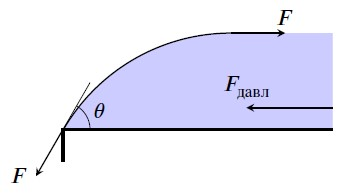
\includegraphics[width=0.4\textwidth]{Figures/Fig 2S1.jpg}
\end{wrapfigure}

\noindent\textbf{1.} Vì $\sqrt{\sigma/(\rho g)}\ll S$, bề mặt của lớp thuỷ ngân dừng như là phẳng và bán kính của lớp thuỷ ngân lớn hơn rất nhiều so với độ dày của nó. Giả sử thuỷ ngân đã che phủ hoàn toàn đáy trên của hình trụ nhưng không tràn xuống mặt bên của nó. Xét một lớp chất lỏng có độ rồng $L$, cân bằng lực theo phương ngang cho:
\begin{equation*}
  F\cos\theta-F+p_{cp}Lh=\sigma L\cos\theta-\sigma L+p_{cp}Lh=0
\end{equation*}
trong đó $p_{cp}$ là áp suất thuỷ tĩnh trung bình theo độ dày của lớp thuỷ ngân:
\begin{equation*}
  p_{cp}=\frac{\rho gh}{2}
\end{equation*}
do đó:
\begin{equation*}
  \frac{\rho gh^{2}}{2}=\sigma(1-\cos\theta)\implies h=\sqrt{\frac{2\sigma(1-\cos\theta)}{\rho g}}
\end{equation*}
khi thuỷ ngân che phủ toàn bộ đáy trên của hình trụ, thể tích của nó bằng:
\begin{equation*}
  V_{0}=Sh=S\sqrt{\frac{2\sigma(1-\cos\theta)}{\rho g}}
\end{equation*}



\noindent\textbf{2.} Nếu đặt lên lớp thuỷ ngân một hình trụ có khối lượng $m$, áp suất thuỷ tĩnh tại mỗi điểm bên trong lớp thuỷ ngân sẽ tăng lên một lượng $mg/S_{k}$ với $S_{k}$ là diện tích tiếp xúc giữa thuỷ ngân và đáy dưới của hình trụ mà ta đặt lên. Áp suất thuỷ tĩnh trung bình trong lớp thuỷ ngân khi này:
\begin{equation*}
  p_{cp}=\frac{\rho gh}{2}+\frac{mg}{S_{k}}
\end{equation*}
điều kiện cân bằng:
\begin{equation*}
  \sigma(1-\cos\theta)=\frac{\rho gh^{2}}{2}+\frac{mgh}{S_{k}}
\end{equation*}
trong đó $h=V/S_{k}$ vì lớp thuỷ cân gần như là phẳng. Ta có:
\begin{equation*}
  \sigma(1-\cos\theta)=\frac{\rho gV^{2}}{2S_{k}^{2}}+\frac{mgV}{S_{k}^{2}}
\end{equation*}
thuỷ ngân sẽ lấp đầy hoàn toàn khe hở khi $S=S_{k}$, tức:
\begin{equation*}
  m_{1}=\frac{\sigma S^{2}(1-\cos\theta)}{gV}-\rho V^{2}
\end{equation*}

\begin{figure}[h]
  \centering
  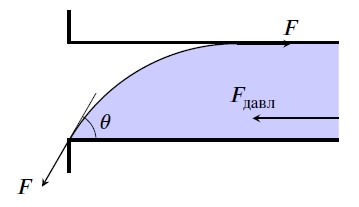
\includegraphics[width=0.4\textwidth]{Figures/Fig 2S2.jpg}
\end{figure}

\noindent\textbf{3.} Trong quá trình thuỷ ngân tràn ra bên ngoài, tiếp tuyến của bề mặt thuỷ ngân sẽ quay $90^{\circ}$. Thuỷ ngân sẽ bắt đầu tràn ra khỏi khe hở khi áp suất thuỷ tĩnh vượt quá giá trị cho phép của lực căng bề mặt theo phương ngang. Xét hai trường hợp:
\begin{figure}[h]
  \centering
  \begin{subfigure}[b]{0.49\textwidth}
    \centering
    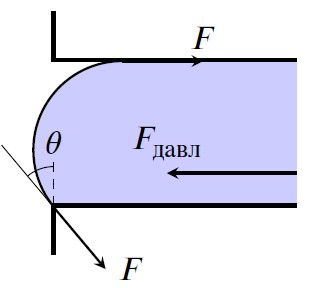
\includegraphics[width=0.8\textwidth]{Figures/Fig 2S3.jpg}
    \caption{Trường hợp 1}
  \end{subfigure}
  \hfill
  \begin{subfigure}[b]{0.49\textwidth}
    \centering
    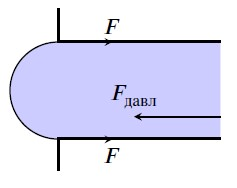
\includegraphics[width=0.7\textwidth]{Figures/Fig 2S4.jpg}
    \caption{Trường hợp 2}
  \end{subfigure}
\end{figure}

\begin{enumerate}
  \item Trường hợp 1: $\theta<\dfrac{\pi}{2}$:\\
        Trong trường hợp này, tiếp tuyến của bề mặt thuỷ ngân sẽ không bao giờ nằm ngang, do đó, độ lớn lực căng bề mặt theo phương ngang sẽ đạt giá trị cực đại khi đường tiếp tuyến hợp một góc $\theta$ với mặt bên của hình trụ. Khi đó:
        \begin{equation*}
          F_{max}=\sigma L(1+\sin\theta)
        \end{equation*}
        như đã chỉ ra ở trên, điều kiện cân bằng là:
        \begin{equation*}
          \sigma(1+\sin\theta)=\frac{\rho gV^{2}}{2S^{2}}+\frac{m_{2}gV}{S^{2}}
        \end{equation*}
        suy ra:
        \begin{equation*}
          m_{2}=\frac{\sigma S^{2}(1+\sin\theta)}{gV}-\rho V^{2}
        \end{equation*}
  \item Trường hợp 2: $\theta\geqslant\dfrac{\pi}{2}$:
        Trong trường hợp này, tiếp tuyến của bề mặt thuỷ ngân có thể nằm theo phương ngang. Khi đó, độ lớn lực căng bề mặt theo phương ngang sẽ có giá trị cực đại:
        \begin{equation*}
          F_{max}=2\sigma L
        \end{equation*}
        lập luận tương tự trường hợp 1, ta được:
        \begin{equation*}
          m_{2}=\frac{2\sigma S^{2}}{gV}-\rho V^{2}
        \end{equation*}
\end{enumerate}


